\documentclass[../MasterThesis.tex]{subfiles}
\graphicspath{ {./assets/images/} }


%----------------------------------------------------------------------------
%----------------------------------------------------------------------------

\begin{document}
	
	
%
%
%
%
%=======================================================================================================
%
%
%
%
%=======================================================================================================
% CHAPTER: CONCLUSION AND FUTURE WORK
%=======================================================================================================
\newpage
\section{Conclusion} \label{section:conclusion}


%-------------------------------------------------------------------------------------------------------
\subsection{Summary, Contributions and Limitations} \label{subsection:summary}
% Summarize the key findings and outcomes of the research.




%-------------------------------------------------------------------------------------------------------
\subsection{Future Work} \label{subsection:futurework}
% Suggest possible extensions or improvements to your work.


TODO


%-------------------------------------------------------------------------------------------------------
\subsubsection*{Video Presets}

Video presets, also known as video filters or video effects, are pre-configured settings or adjustments that can be applied to videos to achieve specific visual styles or effects. 
These presets often include templates for colour grading. 
Video presets are commonly used in video editing software and social media platforms. They provide the user with options to customize their videos easily. 

One example for video presets can be seen in Figure~\ref{figure:app}, where the presets in Adobe Premiere Pro with the \textit{Magic Bullet Looks} plug-in are shown.~\cite{premierepro, magicbullet}

\begin{figure}[H]
	
	\centering
	
	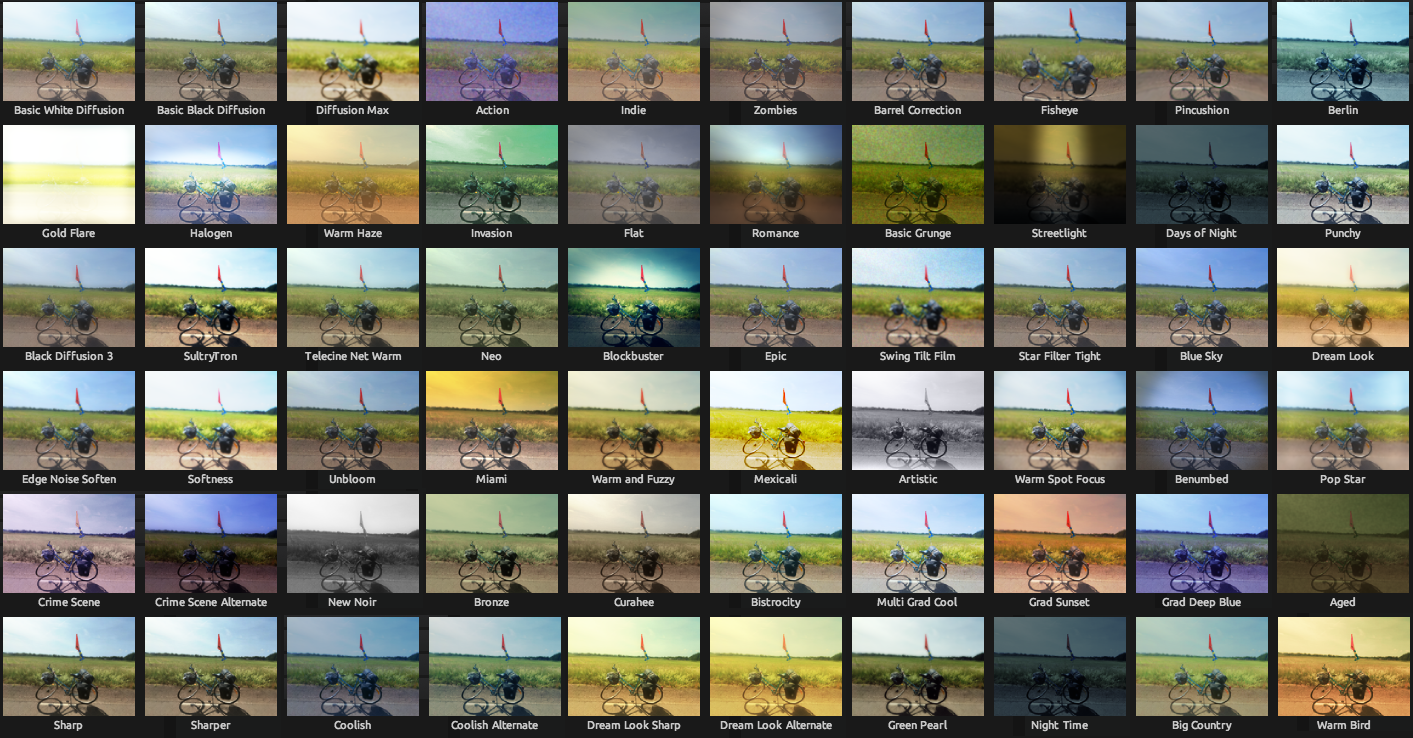
\includegraphics[width=0.99\textwidth]{app.png}
	
	\caption[Presets in Adobe Premiere Pro (\textit{Magic Bullet Looks})]{Presets in Adobe Premiere Pro with the plug-in \textit{Magic Bullet Looks}~\cite{premierepro, magicbullet}}
	\label{figure:app}
	
\end{figure}

Implementing options for the application of those presets is an interesting opportunity for future work. To implement this, different Melt filters can be used or combined. Different options for those Melt filters can be seen in Appendix~\ref{appendix:differentMeltFilter}.

The implementation and usage of those video presets needs a new design for the user interface, to guarantee the usability. TODO












%-------------------------------------------------------------------------------------------------------
\subsubsection*{Audio filter}

This thesis project focussed on the application of visual filters to a video, especially the adjustment of the RGB values. Aside from this, audio processing plays a role in the processing of videos, too. Similar to the visual content, the audio can enhance the experience and evoke emotions in the viewer. Audio filters can also be used to improve the quality of the recorded audio for example by applying noise suppression or to add context to a scene, by adding fitting surrounding noises. In addition to this, simple aspects including the volume or tone can be modified.
The list of filters on the Melt website contains the available audio filters, too.~\cite{melt}

The implementation of the audio filter integrations is an interesting option for future work. To compare different audio filters, the according sound waves of a track could be read out and compared.









%-------------------------------------------------------------------------------------------------------
\subsubsection*{Improvements in the User Interface}


TODO

\begin{itemize}
	\item Including User Feedback and Testing
\end{itemize}








%-------------------------------------------------------------------------------------------------------
\subsubsection*{Advanced Video Processing}

TODO 

\begin{itemize}
	\item Advanced Colour Grading Techniques
	\item Online Video Editing Tool
\end{itemize}








	
	
	
\end{document}